\documentclass[svgnames,11pt]{standalone}
\usepackage[utf8]{inputenc}
\usepackage[T1]{fontenc}
\usepackage{csquotes}
\usepackage[english]{babel}
\usepackage{xcolor}
\usepackage{charter}
\usepackage{amsmath}
\usepackage{amssymb}
\usepackage[np,autolanguage]{numprint}
\newcommand{\outqt}[1]{{\textcolor{DarkOrange}{#1}}}
\newcommand{\inqt}[1]{{\textcolor{Blue}{#1}}}
\usepackage{tikz}
\usetikzlibrary{arrows,automata,calc}
\usetikzlibrary{arrows.meta}
\usetikzlibrary{decorations.pathreplacing}
\usetikzlibrary{backgrounds,shapes}
\tikzset{%
  show curve controls/.style={
    postaction={
      decoration={
        show path construction,
        curveto code={
          \draw [blue] 
            (\tikzinputsegmentfirst) -- (\tikzinputsegmentsupporta)
            (\tikzinputsegmentlast) -- (\tikzinputsegmentsupportb);
          \fill [red, opacity=0.5] 
            (\tikzinputsegmentsupporta) circle [radius=.25ex]
            (\tikzinputsegmentsupportb) circle [radius=.25ex];
        }
      },
      decorate
}}}
\tikzstyle{vertex}=[draw,circle,black,inner sep=2pt]
\tikzstyle{edge}=[line width=1.3pt,color=Black]
\tikzstyle{rare}=[fill=black,text=white]
\tikzstyle{medium}=[fill=black!15!white]


\newcommand{\epslabel}{{$2$}}
\usepackage{fixltx2e,graphicx}
\newcommand{\unaryminus}{\scalebox{0.5}[1.0]{\(-\)}}
\newcommand{\minuslabel}{{$\unaryminus1$}}

\begin{document}
       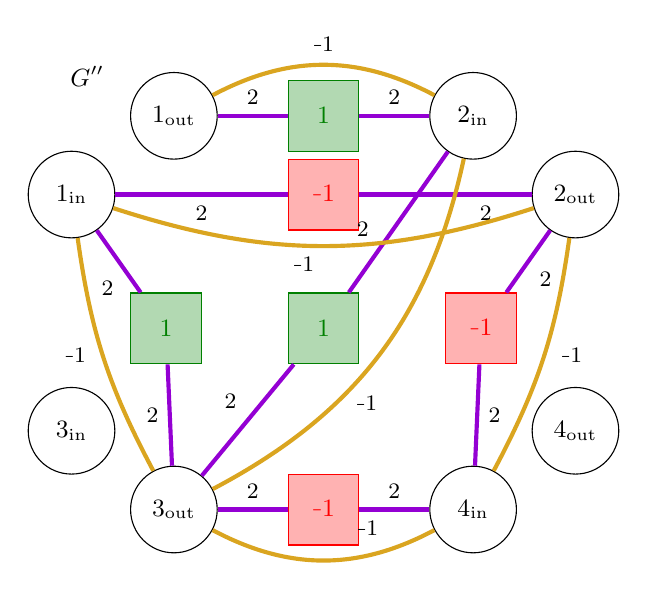
\begin{tikzpicture}[auto, every node/.style={transform shape}]
         \tikzset{>=latex}
         \tikzstyle{peers}=[font=\small,draw,circle,black,minimum width=11mm,inner sep=0,fill opacity=.0, text opacity=1]
         \tikzstyle{nedge}=[font=\small,draw,rectangle,black,minimum width=9mm,minimum height=9mm, inner sep=0]
         \tikzstyle{uedge}=[line width=1.5pt,color=Black]
         \tikzstyle{edge}=[uedge,-{Latex[length=4mm,width=1.5mm,angle'=40]}]
         \tikzstyle{pnode}=[fill=White]
         \tikzstyle{elabel}=[color=Black,font=\footnotesize]
         \tikzstyle{qnode}=[fill=White]
         \tikzstyle{posc}=[color=Green, fill=Green!30!white]
         \tikzstyle{negc}=[color=red, fill=red!30!white]
         \tikzstyle{neuc}=[color=black!80!white, fill=black!30!white]
         \tikzstyle{eps}=[color=DarkViolet]
         \tikzstyle{minus}=[color=Goldenrod]

         \node[peers,pnode] (p1) at (1.3, -1.0) {$1_{\mathrm{out}}$}; 
         \node[peers,pnode] (p2) at (6.4, -2.0) {$2_{\mathrm{out}}$}; 
         \node[peers,pnode] (p3) at (1.3, -6.0) {$3_{\mathrm{out}}$}; 
         \node[peers,pnode] (p4) at (6.4, -5.0) {$4_{\mathrm{out}}$}; 
         \node[peers,qnode] (q1) at (0.0, -2.0) {$1_{\mathrm{in}}$}; 
         \node[peers,qnode] (q2) at (5.1, -1.0) {$2_{\mathrm{in}}$}; 
         \node[peers,qnode] (q3) at (0.0, -5.0) {$3_{\mathrm{in}}$}; 
         \node[peers,qnode] (q4) at (5.1, -6.0) {$4_{\mathrm{in}}$}; 
         \node[nedge,posc]  (e1) at (3.2, -1.0) {$1$}; 
         \node[nedge,negc]  (e2) at (3.2, -2.0) {$\unaryminus1$}; 
         \node[nedge,negc]  (e3) at (5.2, -3.7) {$\unaryminus1$}; 
         \node[nedge,posc]  (e4) at (1.2, -3.7) {$1$}; 
         \node[nedge,posc]  (e5) at (3.2, -3.7) {$1$}; 
         \node[nedge,negc]  (e6) at (3.2, -6.0) {$\unaryminus1$};
         \node[] (caption) at (0.2, -.5) {\small $G''$};

         \draw[uedge,eps] (p1) edge [bend left=0] node [elabel,]               {\epslabel} (e1);
         \draw[uedge,eps] (p2) edge [bend left=0] node [elabel,pos=.25]       {\epslabel} (e2);
         \draw[uedge,eps] (e2) edge [bend left=0] node [elabel,]               {\epslabel} (q1);
         \draw[uedge,eps] (p2) edge [bend left=0] node [elabel,]               {\epslabel} (e3);
         \draw[uedge,eps] (e3) edge [bend left=0] node [elabel,]               {\epslabel} (q4);
         \draw[uedge,eps] (e4) edge [bend left=0] node [elabel,pos=.35]       {\epslabel} (q1);
         \draw[uedge,eps] (e6) edge [bend left=0] node [elabel,]               {\epslabel} (q4);
         \draw[uedge,eps] (p3) edge [bend left=0] node [elabel,]                {\epslabel} (e4);
         \draw[uedge,eps] (p3) edge [bend left=0] node [elabel,]               {\epslabel} (e5);
         \draw[uedge,eps] (p3) edge [bend left=0] node [elabel,]               {\epslabel} (e6);
         \draw[uedge,eps] (e1) edge [bend left=0] node [elabel,]               {\epslabel} (q2);
         \draw[uedge,eps] (e5) edge [bend left=0] node [elabel,pos=0.3]       {\epslabel} (q2);

         \draw[uedge,minus] (p1) edge [bend left=28] node  [elabel,]          {\minuslabel} (q2);
         \draw[uedge,minus] (p2) edge [bend left=18] node  [elabel,pos=.55]   {\minuslabel} (q1);
         \draw[uedge,minus] (p2) edge [bend left=10] node  [elabel,pos=.4]    {\minuslabel} (q4);
         \draw[uedge,minus] (p3) edge [bend left=10] node  [elabel,pos=.6]     {\minuslabel} (q1);
         \draw[uedge,minus] (p3) edge [bend left=-25] node [elabel,pos=0.45,below=5pt] {\minuslabel} (q2);
         \draw[uedge,minus] (p3) edge [bend right=28] node [elabel,pos=.8]           {\minuslabel} (q4);
       \end{tikzpicture}
\end{document}
